\section{The case $[2 \times 3, 6]_4$}
\begin{lemma}
  Let $p = (p_3, p_4, p_5, \dots, p_n)$ be a given sequence satisfying equation \ref{eq_valence_4} as well as $p_4 \leq 3$, $p_5 \leq 3$ and $3 \mid 2 \sum_{k=3}^{n} p_k - 4$. Then there exists $r \in \nats$ for which $p + r [2 \times 3, 6]_3$ is $4$-realizable.

  All the requirements in the statement will help utilizing Eberhards Theorem \ref{thm_eberhard}(\ref{thm_eberhard_3}). The conditions $p_4 \leq 3$, $p_5 \leq 3$ deal with different sign of curvatures when having valence $3$ and $4$ (note that quadrangles and pentagons have positive curvature in the case of $3$-valence but zero or negative curvature in the other case), while the condition $p_4 \leq 3$, $p_5 \leq 3$ is necessary to keep the number of triangles natural. 
  \begin{proof}
    One can restate \ref{eq_valence_4} to a form looking more like \ref{eq_valence_3}:
    \begin{align*}
      & \sum_{k=3}^n \left( 4 - k \right) p_k = 8 \\
      \implies & \sum_{k=3}^n \left( 6 - k \right) p_k - \left(2 \sum_{k=3}^n  p_k - 4 \right) = 12
    \end{align*}
    Let $r_3 := (2 \sum_{k=3}^{n} p_k - 4)/3$. From
    \begin{align*}
      3 r_3 &= 2 \sum_{k=3}^{n} p_k - 4 =  2 p_3 + 2 p_4 + 2 p_5 + \sum_{k=6}^{n} p_k - 4\\
      \implies r_3 &= 2 p_4 + 2 p_5 - 4 + \sum_{k=6}^{n} p_k \leq 8 + 2 \sum_{k=6}^{n} p_k \leq 8 + \sum_{k=4}^{n} (k - 4) p_k = p_3
    \end{align*}
    follows, that $p_3' := p_3 - r_3 \geq 0$ and setting $p_k' := p_k$, $(k \geq 4)$ the resulting sequence $p'$ suffices \ref{eq_valence_3}. Using \ref{thm_eberhard}(\ref{thm_eberhard_3}) one get a $3$-realization $P'$ of $p'$. Inserting in $P'$ an hexagon for every edge and four triangles for every vertex as seen in the following figure one can construct a $4$-realization of some sequence $p''$.
    \begin{figure}[htpp]
      \centering
      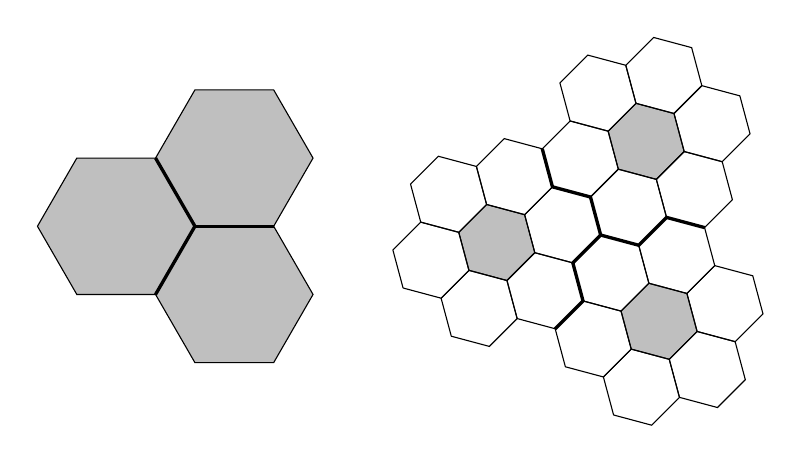
\begin{tikzpicture}
        \matrix (m) [ column sep=1cm] {
          \begin{scope}[xscale=1.0, yscale=0.866]
            \filldraw[fill=gray!50!white] (0, 1) -- ++(0.5, -1) -- ++(1, 0) -- ++(0.5, 1) -- ++(-0.5, 1) -- ++(-1, 0) -- ++(-0.5, -1);
            \filldraw[fill=gray!50!white] (1.5, 0) -- ++(0.5, -1) -- ++(1, 0) -- ++(0.5, 1) -- ++(-0.5, 1) -- ++(-1, 0) -- ++(-0.5, -1);
            \filldraw[fill=gray!50!white] (1.5, 2) -- ++(0.5, -1) -- ++(1, 0) -- ++(0.5, 1) -- ++(-0.5, 1) -- ++(-1, 0) -- ++(-0.5, -1);
            \draw[very thick] (1.5, 0) -- ++(0.5, 1) -- ++(-0.5, 1);
            \draw[very thick] (2, 1) -- ++(1, 0);
          \end{scope}
          &


          \begin{scope}[rotate=45, xscale=1.0, yscale=0.866, scale=0.5] 
            \filldraw[fill=gray!50!white] (0, 1) -- ++(0.5, -1) -- ++(1, 0) -- ++(0.5, 1) -- ++(-0.5, 1) -- ++(-1, 0) -- ++(-0.5, -1);
            \draw (-1.5, 0) -- ++(0.5, -1) -- ++(1, 0) -- ++(0.5, 1) -- ++(-0.5, 1) -- ++(-1, 0) -- ++(-0.5, -1);
            \draw (0, -1) -- ++(0.5, -1) -- ++(1, 0) -- ++(0.5, 1) -- ++(-0.5, 1) -- ++(-1, 0) -- ++(-0.5, -1);
            \draw (1.5, 0) -- ++(0.5, -1) -- ++(1, 0) -- ++(0.5, 1) -- ++(-0.5, 1) -- ++(-1, 0) -- ++(-0.5, -1);
            \draw (1.5, 2) -- ++(0.5, -1) -- ++(1, 0) -- ++(0.5, 1) -- ++(-0.5, 1) -- ++(-1, 0) -- ++(-0.5, -1);
            \draw (0, 3) -- ++(0.5, -1) -- ++(1, 0) -- ++(0.5, 1) -- ++(-0.5, 1) -- ++(-1, 0) -- ++(-0.5, -1);
            \draw (-1.5, 2) -- ++(0.5, -1) -- ++(1, 0) -- ++(0.5, 1) -- ++(-0.5, 1) -- ++(-1, 0) -- ++(-0.5, -1);

            \filldraw[fill=gray!50!white] (4.5, 0) -- ++(0.5, -1) -- ++(1, 0) -- ++(0.5, 1) -- ++(-0.5, 1) -- ++(-1, 0) -- ++(-0.5, -1);
            \draw (3, -1) -- ++(0.5, -1) -- ++(1, 0) -- ++(0.5, 1) -- ++(-0.5, 1) -- ++(-1, 0) -- ++(-0.5, -1);
            \draw (4.5, -2) -- ++(0.5, -1) -- ++(1, 0) -- ++(0.5, 1) -- ++(-0.5, 1) -- ++(-1, 0) -- ++(-0.5, -1);
            \draw (6, -1) -- ++(0.5, -1) -- ++(1, 0) -- ++(0.5, 1) -- ++(-0.5, 1) -- ++(-1, 0) -- ++(-0.5, -1);
            \draw (6, 1) -- ++(0.5, -1) -- ++(1, 0) -- ++(0.5, 1) -- ++(-0.5, 1) -- ++(-1, 0) -- ++(-0.5, -1);
            \draw (4.5, 2) -- ++(0.5, -1) -- ++(1, 0) -- ++(0.5, 1) -- ++(-0.5, 1) -- ++(-1, 0) -- ++(-0.5, -1);
            \draw (3, 1) -- ++(0.5, -1) -- ++(1, 0) -- ++(0.5, 1) -- ++(-0.5, 1) -- ++(-1, 0) -- ++(-0.5, -1);
            
            \filldraw[fill=gray!50!white] (1.5, -4) -- ++(0.5, -1) -- ++(1, 0) -- ++(0.5, 1) -- ++(-0.5, 1) -- ++(-1, 0) -- ++(-0.5, -1);
            \draw (0, -5) -- ++(0.5, -1) -- ++(1, 0) -- ++(0.5, 1) -- ++(-0.5, 1) -- ++(-1, 0) -- ++(-0.5, -1);
            \draw (1.5, -6) -- ++(0.5, -1) -- ++(1, 0) -- ++(0.5, 1) -- ++(-0.5, 1) -- ++(-1, 0) -- ++(-0.5, -1);
            \draw (3, -5) -- ++(0.5, -1) -- ++(1, 0) -- ++(0.5, 1) -- ++(-0.5, 1) -- ++(-1, 0) -- ++(-0.5, -1);
            \draw (3, -3) -- ++(0.5, -1) -- ++(1, 0) -- ++(0.5, 1) -- ++(-0.5, 1) -- ++(-1, 0) -- ++(-0.5, -1);
            \draw (1.5, -2) -- ++(0.5, -1) -- ++(1, 0) -- ++(0.5, 1) -- ++(-0.5, 1) -- ++(-1, 0) -- ++(-0.5, -1);
            \draw (0, -3) -- ++(0.5, -1) -- ++(1, 0) -- ++(0.5, 1) -- ++(-0.5, 1) -- ++(-1, 0) -- ++(-0.5, -1);

            \draw[very thick] (0.5, -2) -- ++(1, 0) -- ++(0.5, 1) -- ++(1, 0) -- ++(0.5, 1) -- ++(-0.5, 1) -- ++(0.5, 1);
            \draw[very thick] (3, -1) -- ++(0.5, -1) -- ++(1, 0) -- ++(0.5, -1);
          \end{scope};
          \\
        };
      \end{tikzpicture}
    \end{figure}

  \end{proof}
  
\end{lemma}

\begin{theorem}
  Let $p = (p_3, p_4, p_5, \dots, p_n)$ and $q = (q_3, q_4, q_5, \dots, q_n)$ be a given sequences both of which are 4-realizable. Then their ``sum'', $(p_3 + q_3 - 8, p_4 + q_4, ..., p_n + q_n)$ is also 4-realizable.
  \begin{proof}
  \end{proof}
\end{theorem}


